\chapter{Ergebnisse}\label{chap:results}
%\begin{itemize}
%	\item Hyperparameter beschreiben (Clients pro Runde, Learning Rate yadayadayada)
%	\item Numerisch beschreiben was es für Unterschiede gibt (bei iid ist das Delta von der Privacy setups so und so usw)
%	\item $\delta$'s pro Datensatz erwähnen und sagen wie ich sie gewählt habe
%\end{itemize}

In diesem Kapitel gehe ich auf die Ergebnisse der Experimente aus \autoref{chap:experiments} ein. In \autoref{sec:non-fl-training-results} beschreibe ich Ergebnisse von lokalen Trainingsdurchläufen mit dem identischen Modell. In \autoref{sec:fl-training-results} erläutere ich detaillierter, welche Ergebnisse ich im Federated Learning erzielt habe und beschreibe die genutzten Hyperparameter.

\section{Non-federated Training} \label{sec:non-fl-training-results}
Die Ergebnisse der lokalen Trainingsdurchläufe sind, wie zu erwarten, etwas besser als im Federated Learning, auch wenn sie nicht der \textit{state-of-the-art} entsprechen. Das liegt an dem einfachen und kleinen Modell, das ich für das Training genutzt habe.

Bei MNIST und SVHN erreicht das Modell bereits innerhalb von 10 Epochen gute Ergebnisse. Bei CIFAR-10 sind die Ergebnisse deutlich schlechter, weshalb ich hier mit einem \texttt{EarlyStopping}-Callback gearbeitet habe, der abbricht sobald das Modell \textit{overfittet}. Trotzdem liegt die erreichte Accuracy unter 50\%. Eine Übersicht zeigt \autoref{tab:local-model-results}.

\begin{table}
	\centering
	\begin{tabular}{ccc}
		\toprule
		Dataset & Accuracy & Loss \\
		\midrule
		MNIST & 0.9842 & 0.0535 \\
		SVHN & 0.8758 & 0.4203 \\
		CIFAR-10 & 0.634 & 1.0395 \\
		\bottomrule
	\end{tabular}
	\caption{Die Ergebnisse von nicht privaten und zentral durchgeführten Trainingsdurchläufen}
	\label{tab:local-model-results}
\end{table}

Allerdings liegt der Fokus meiner Arbeit auf dem Federated Learning Algorithmus und die lokalen Trainingsdurchläufe sollten vor allem zum Vergleich und zum Finden von angemessenen Modellen und Hyperparametern dienen. Sie waren hilfreich, denn ich konnte beispielsweise mein Convolutional Neural Network mit einem Feed-Forward Netz vergleichen. 

Die Trainingszeit liegt bei wenigen Sekunden oder Minuten. Derartige Experimente wären im Federated Learning sehr viel umständlicher gewesen, da das Training einen deutlich erhöhten Rechenaufwand mit sich bringt und auch, was die Konvergenz der Modelle betrifft, instabiler ist.

\begin{figure}
	\centering
	\begin{subfigure}{0.32\textwidth}
		\centering
		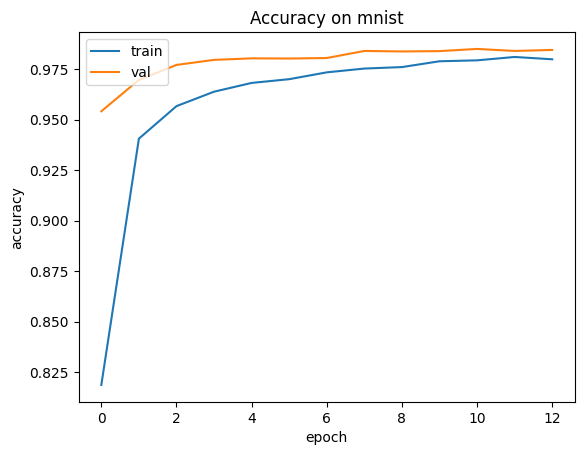
\includegraphics[width=\textwidth]{Bilder/mnist-results-local.png}
		\caption{MNIST}
	\end{subfigure}
	\begin{subfigure}{0.32\textwidth}
		\centering
		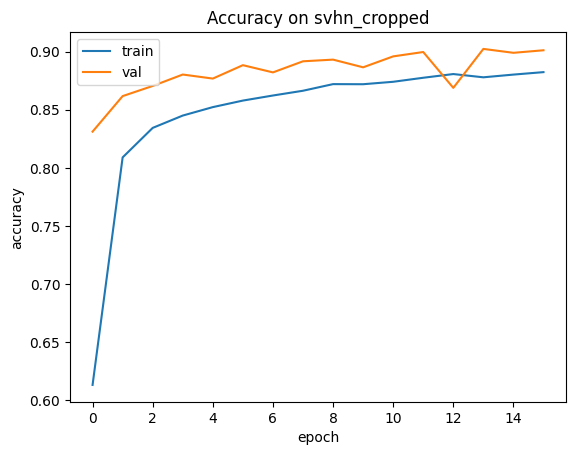
\includegraphics[width=\textwidth]{Bilder/svhn-results-local.png}
		\caption{SVHN}
	\end{subfigure}
	\begin{subfigure}{0.32\textwidth}
		\centering
		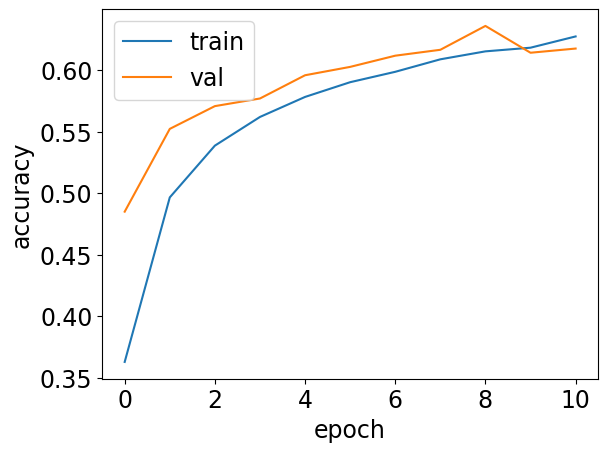
\includegraphics[width=\textwidth]{Bilder/cifar-results-local.png}
		\caption{CIFAR-10}
	\end{subfigure}
	\caption{Genauigkeiten auf den Trainings- und Validierungsdatensätzen im nicht-privaten, zentralen Training}
	\label{fig:local-training-histories}
\end{figure}

\section{Federated Training}\label{sec:fl-training-results}

Die Ergebnisse des Trainings im Federated Learning sind in \autoref{tab:all-fed-results} zu sehen. Die Ergebnisse sind nach den Datensätzen aufgeteilt und jeweils für die normale Version (\textit{non-i.i.d.}) und die unabhängig gleichverteilte Version (\textit{i.i.d.}) notiert. Die gleichverteilte Version ist durch das in \autoref{sec:iid-dataset-creation} beschriebene Verfahren entstanden.

Die Genauigkeit bezieht sich in jedem Fall auf die Auswertung des Modells auf den Testdaten. Für die Evaluierung habe ich die Testdaten zu einem zentralen Datensatz zusammengefügt und dann das Modell darauf evaluiert. Eine andere Möglichkeit wäre gewesen, die Evaluierung ebenfalls auf den Clients durchzuführen. Für den Fall, dass man ein vortrainiertes Modell für jeden Client noch einmal nachtrainiert, damit es auf seinen Daten gut funktioniert, wäre diese Art der Evaluierung angemessener gewesen. Allerdings war ich nur an der allgemeinen Performanz des Modells interessiert.

Es ist auffällig, dass die Modelle auf allen Datensätzen in der gleichverteilten Version besser abschneiden. Das deckt sich mit dem Stand der Forschung zu \texttt{FedAvg}.

\begin{table}
	\centering
	\begin{tabular}{lp{4em}p{4em}p{4em}p{4em}p{4em}p{4em}}
		\toprule 
	 	& \multicolumn{2}{c}{MNIST} & \multicolumn{2}{c}{SVHN} & \multicolumn{2}{c}{CIFAR-10} \\
		\cmidrule(lr){2-3}\cmidrule(lr){4-5}\cmidrule(lr){6-7}
		& i.i.d. & non-i.i.d. & i.i.d. & non-i.i.d. & i.i.d. & non-i.i.d. \\
		\midrule
		\texttt{no-dp} & 0.906 & 0.896 & 0.825 & - & 0.419 & 0.246 \\
		\texttt{relaxed-dp} & 0.931 & 0.855 & 0.544 & - & 0.407 & 0.252 \\
		\texttt{relaxed-idp} & 0.917 & 0.883 & 0.418 & - & 0.394 & 0.255 \\
		\texttt{strict-idp} & 0.91 & 0.887 & 0.446 & - & 0.386 & 0.235 \\
		\texttt{strict-dp} & 0.895 & 0.811 & 0.292 & - & 0.387 & 0.246 \\
		\bottomrule
	\end{tabular}
	\caption{Mit den verschieden Privacy Setups erzielte Genauigkeiten im Federated Training}
	\label{tab:all-fed-results}
\end{table}

\subsection{Hyperparameter Setups}
Ich habe das Training mit allen Datensätzen auf $100$ Runden begrenzt. Grund dafür war einerseits die Trainingszeiten kurz zu halten, andererseits gibt es auch eine Wechselwirkung mit der Anzahl der Runden und dem Privacy Loss. Bei einer höheren Rundenzahl erhöht er sich, denn jeder Client wird im Verlauf des Trainings häufiger oder mit einer größeren Wahrscheinlichkeit gezogen. Daher muss im Umkehrschluss das Rauschen größer werden. 

Ein weiterer Hyperparameter, der einen Einfluss auf die Stärke des Rauschens hat, ist die Anzahl der Clients, die pro Runde gezogen werden sollen. Davon hängt die Wahrscheinlichkeit mit der die Clients gezogen werden ab. Hier gilt ebenso, dass bei einer größeren Wahrscheinlichkeit die Daten eines Clients einen größeren Einfluss auf das trainierte Modell haben und damit das Rauschen vergrößert werden muss.

Hyperparameter, die sich nicht auf den Privacy Loss auswirken sind die Learning Rates auf dem Server und die Learning Rates auf den Clients. Auch die Anzahl der Epochen, die jeder Client auf seinen Daten trainiert, und die Größe der Batches wirken sich nicht auf den Privacy Loss aus.

Wie in \autoref{chap:methods} beschrieben, verwende ich für die Hyperparameter des \textit{Adaptive Clippings} die Standardwerte.

\begin{table}[tb]
	\centering
	\begin{tabular}{lccc}
		\toprule
		Hyperparameter & MNIST & SVHN & CIFAR-10 \\
		\midrule
		Rounds & 100 & 100 & 100 \\
		Clients per round & 50 & 30 & 30 \\
		Batchsize & 128 & 128 & 128 \\
		Local Epochs & 5 & 5 & 5 \\
		Client learning rate & 0.001 & 0.001 & 0.001 \\
		Server learning rate & 1.0 & 1.0 & 1.0 \\
		\bottomrule
	\end{tabular}
	\caption{Hyperparameter, die auf den verschiedenen Datensätzen genutzt wurden}
	\label{tab:fl-hyperparameters}
\end{table}

\subsection{MNIST}

Bei MNIST konnten die DP-Algorithmen ähnlich gute Ergebnisse erzielen wie das nicht-private \texttt{FedAvg}. In \autoref{fig:fed-emnist-results} ist dennoch ein Einfluss des Privacy Setups auf das Ergebnis zu sehen. Vor allem \texttt{strict-dp} konvergiert ein bisschen instabiler und kommt nicht ganz an die anderen Ergebnisse heran. Außerdem fällt der Loss bei \texttt{no-dp} bereits deutlich früher ab. Bei den anderen Setups erfolgt die Absenkung erst nach ungefähr 15 Runden. Die restlichen Privacy-Niveaus liegen sehr nah beieinander, allerdings ist auffällig, dass \texttt{relaxed-dp} schlechter abschneidet, als die individualisierten Niveaus.

\begin{figure}[h]
	\centering
	\begin{subfigure}{0.45\textwidth}
		\centering
		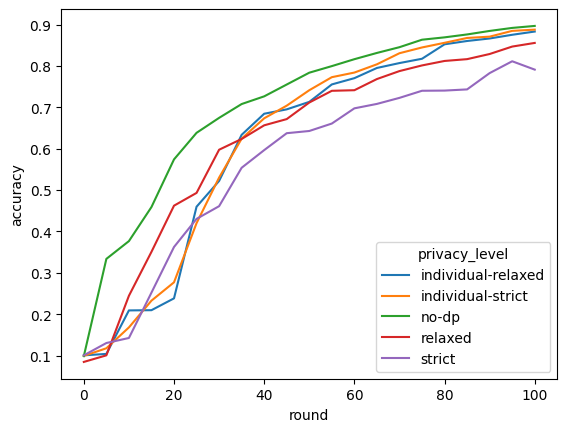
\includegraphics[width=\textwidth]{Bilder/emnist-accuracy.png}
		\caption{Genauigkeit auf Validierungsdaten (non-i.i.d)}
	\end{subfigure}
	\begin{subfigure}{0.45\textwidth}
		\centering
		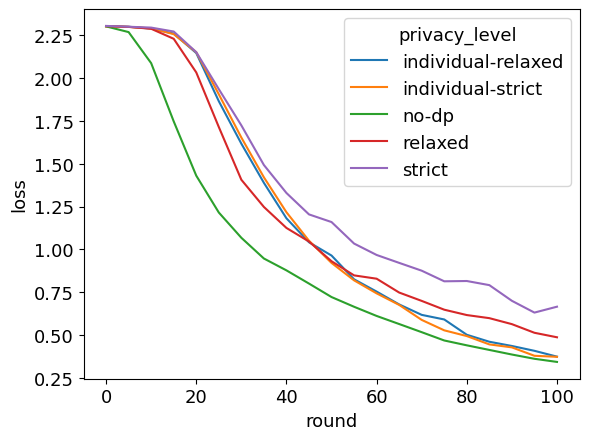
\includegraphics[width=\textwidth]{Bilder/emnist-loss.png}
		\caption{Loss auf Validierungsdaten (non-i.i.d)}
	\end{subfigure}
	\begin{subfigure}{0.45\textwidth}
		\centering
		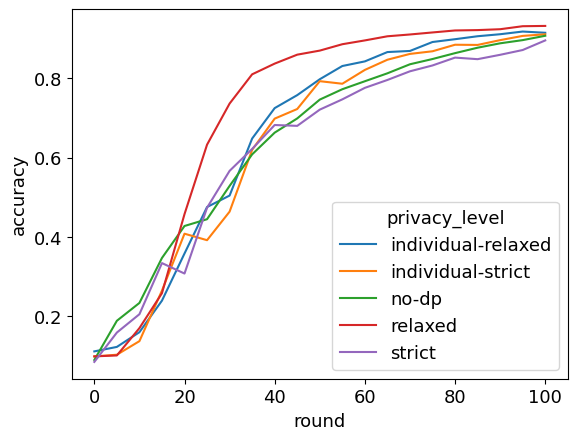
\includegraphics[width=\textwidth]{Bilder/emnist-accuracy-iid.png}
		\caption{Genauigkeit auf Validierungsdaten (i.i.d)}
	\end{subfigure}
	\begin{subfigure}{0.45\textwidth}
		\centering
		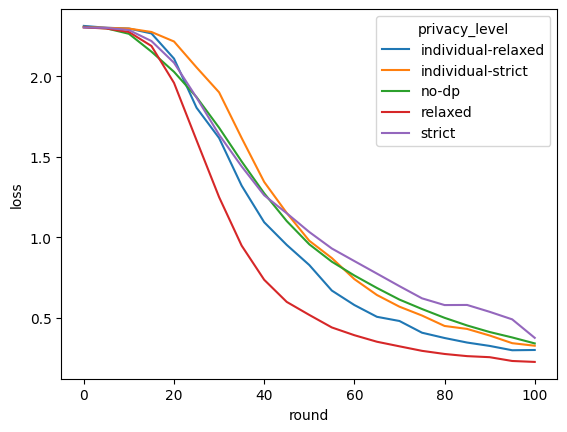
\includegraphics[width=\textwidth]{Bilder/emnist-loss-iid.png}
		\caption{Loss auf Validierungsdaten (i.i.d)}
	\end{subfigure}
	\caption{Genauigkeit und Loss der verschiedenen Privacy Setups im Verlauf des Trainings auf MNIST}
	\label{fig:fed-emnist-results}
\end{figure}

Die vorher berechneten Noise Multiplier für jedes Setup sind in \autoref{tab:noise-multipliers} zu sehen. Wie erwartet sind sie aufsteigend, je nach Größe des Privacy Budgets der Clients.

\begin{table}
	\centering
	\begin{tabular}{lccc}
		\toprule
		Setup & MNIST & SVHN & CIFAR-10 \\
		\midrule
		\texttt{no-dp} & - & - & - \\
		\texttt{relaxed-dp} & 0.769 & 0.348 & 0.384 \\
		\texttt{relaxed-idp} & 0.917 & 0.415 & 0.461 \\
		\texttt{strict-idp} & 1.000 & 0.444 & 0.494 \\
		\texttt{strict-dp} & 1.180 & 0.508 & 0.568 \\
		\bottomrule
	\end{tabular}
	\caption{Noise Multiplier der verschiedenen Setups}
	\label{tab:noise-multipliers}
\end{table}

Bei dem Training auf MNIST konnte ich mit $50$ Clients pro Runde im Erwartungswert gute Ergebnisse erzielen. Zwar würde man erwarten, dass das Modell mit mehr Clients in jeder Runde eine repräsentativere Stichprobe der Daten sieht, allerdings ist die Anzahl der Clients wie beschrieben ein Parameter der auch das Rauschen verstärkt. Daher konnte ich mit größeren Zahlen keine besseren Ergebnisse beobachten.

\subsection{SVHN}

Bei SVHN ist der Unterschied zwischen dem Training mit und ohne Differential Privacy sehr viel deutlicher zu sehen. Während die Metriken sich ohne Differential Privacy im Trainingsprozess kontinuierlich verbessern, hat jedes Setup mit Differential Privacy ab einem bestimmten Punkt im Training Probleme sich weiter zu verbessern. Vor allem \texttt{strict-dp} kann sich nur für kurze Zeit am Anfang verbessern. Bereits \texttt{relaxed-dp} erreicht kaum mehr eine halb so gute Genauigkeit wie das \texttt{no-dp}. Die beiden individualisierten Setups liegen noch ein wenig darunter, liefern allerdings deutlich bessere Ergebnisse als \texttt{strict-dp}. Auffällig ist, dass \texttt{strict-idp} noch ein bisschen besser abschneidet, als \texttt{relaxed-idp}, allerdings kann das Zufall sein.

Die Nähe der individualisierten Niveaus zu \texttt{relaxed-dp} und der Abstand zu \texttt{strict-dp} zeigt hier sehr deutlich den Vorteil der individualisierten Budgets. Während \texttt{relaxed-dp} zwar noch bessere Ergebnisse erzielt, werden hier die Abstriche bei der Privacy der Clients mit den Budgets $\epsilon_1$ bzw. $\epsilon_2$ sehr groß. Andererseits hält \texttt{strict-dp} zwar alle Budgets ein, da auf alle Clients $\epsilon_1$ angewendet wird, allerdings ist hier die Nützlichkeit des Modells stark beeinträchtigt.

Die \textit{Noise Multiplier} sind ebenfalls aufsteigend, allerdings sind sie insgesamt deutlich niedriger als bei MNIST. Dies zeigt, dass dieser Datensatz deutlich anfälliger gegenüber dem Hinzufügen von Rauschen ist und sich die Ergebnisse sehr schnell verschlechtern können.

\begin{figure}
	\centering
	\begin{subfigure}{0.45\textwidth}
		\centering
		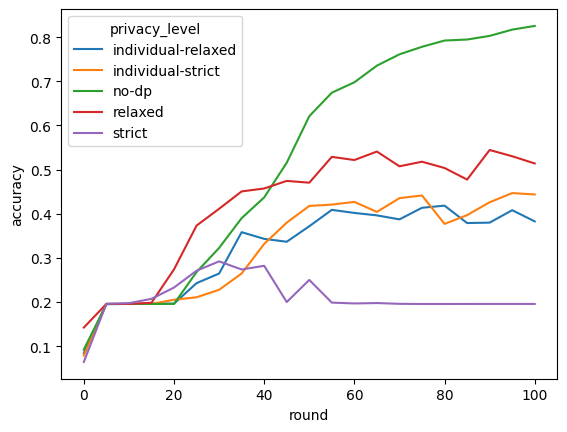
\includegraphics[width=\textwidth]{Bilder/svhn-accuracy.png}
		\caption{Genauigkeit auf Validierungsdaten}
	\end{subfigure}
	\begin{subfigure}{0.45\textwidth}
		\centering
		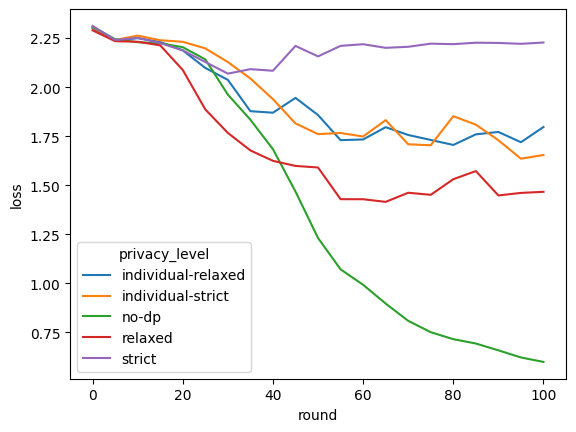
\includegraphics[width=\textwidth]{Bilder/svhn-loss.png}
		\caption{Loss auf Validierungsdaten}
	\end{subfigure}
	\caption{Genauigkeit und Loss der verschiedenen Privacy Setups im Verlauf des Trainings auf SVHN}
	\label{fig:fed-svhn-results}
\end{figure}

\subsection{CIFAR-10}
Bei CIFAR-10 ist auffällig, dass die Performanz des Modells kaum vom Privacy-Niveau abhängt, sondern eher von der Verteilung der Daten. Bei der ungleichmäßigen Verteilung mit dem \textit{Label Distribution Skew} verbessern sich alle Modelle nur sehr langsam und unstetig. Die Unterschiede zwischen den Privacy Niveaus selbst sind kaum zu erkennen.

Bei dem Training auf dem gleichverteilten Datensatz werden alle Modelle deutlich besser. Auch hier liegen die verschiedenen Privacy-Setups nah an dem nicht-privat trainierten Modell. Es fällt aber auf, dass die Verbesserungen der privat trainierten Modelle etwas weniger gleichmäßig ist. Zwischen den individualisierten und den homogenen Budgets ist kein großer Unterschied zu erkennen.

\begin{figure}[tb]
	\centering
	\begin{subfigure}{0.45\textwidth}
		\centering
		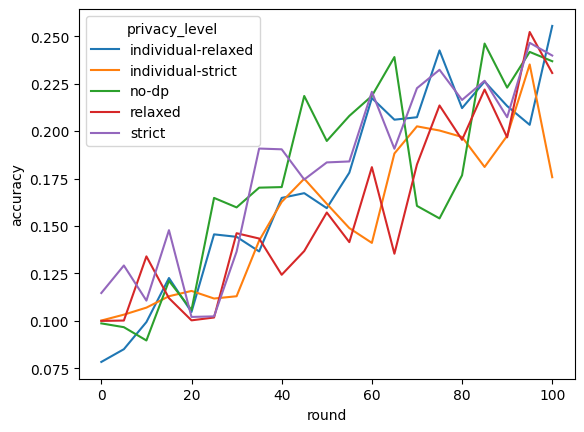
\includegraphics[width=\textwidth]{Bilder/cifar10-accuracy.png}
		\caption{Genauigkeit auf Validierungsdaten (non-i.i.d)}
	\end{subfigure}
	\begin{subfigure}{0.45\textwidth}
		\centering
		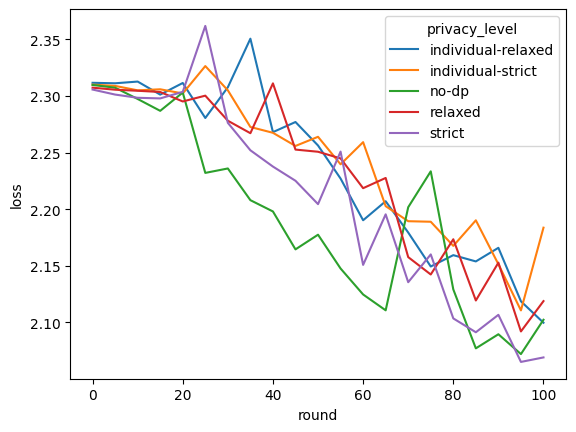
\includegraphics[width=\textwidth]{Bilder/cifar10-loss.png}
		\caption{Loss auf Validierungsdaten (non-i.i.d)}
	\end{subfigure}
	\begin{subfigure}{0.45\textwidth}
		\centering
		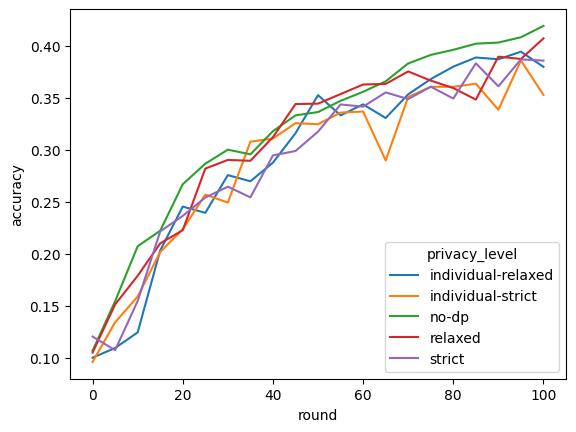
\includegraphics[width=\textwidth]{Bilder/cifar10-accuracy-iid.png}
		\caption{Genauigkeit auf Validierungsdaten (i.i.d)}
	\end{subfigure}
	\begin{subfigure}{0.45\textwidth}
		\centering
		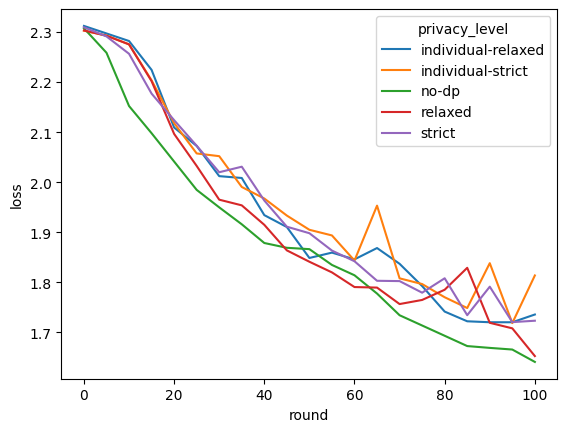
\includegraphics[width=\textwidth]{Bilder/cifar10-loss-iid.png}
		\caption{Loss auf Validierungsdaten (i.i.d)}
	\end{subfigure}
	\caption{Genauigkeit und Loss der verschiedenen Privacy Setups im Verlauf des Trainings auf CIFAR-10}
	\label{fig:fed-cifar10-results}
\end{figure}

\subsection{SVHN und CIFAR-10 mit kleineren Privacy Budgets}

Wie bereits erwähnt habe ich für CIFAR-10 und SVHN deutlich größere Privacy Budgets genutzt als für MNIST. Dies habe ich nicht willkürlich so festgelegt, sondern ich habe nach und nach größere Budgets ausprobiert. In \autoref{fig:cifar-svhn-small-budgets} sind die Trainingsverläufe mit kleineren Privacy Budgets zu sehen.

In der ersten Spalte sind die Trainingsverläufe mit den zu MNIST identischen Budgets von $\epsilon = \{1,2,3\}$ zu sehen. Bei CIFAR-10 fällt auf, dass bei \texttt{strict-dp} keine Verbesserung im Trainingsverlauf stattfindet. Die mit den individualisierten Niveaus trainierten Modelle können sich zunächst etwas verbessern, allerdings sinkt die Validation Accuracy im Verlauf des Trainings wieder.

Auf dem SVHN Datensatz verbessert sich keines der Modelle, die mit Differential Privacy trainiert werden. Alle bleiben beinahe konstant bei einer Genauigkeit von ca. $20\%$, während das nicht-privat trainierte Modell eine Genauigkeit von $80\%$ erreicht. Teilweise bricht die Genauigkeit der privaten Modelle auch immer wieder ein. Das Modell mit dem strengsten Budget (\texttt{strict-dp}) landet sogar bei ungefähr $10\%$, was zufälligem Raten entspricht.

Bei einem höheren Budget von $\epsilon = \{5, 10, 20\}$ entspricht der Trainingsverlauf auf CIFAR-10 deutlich mehr dem Verlauf aus \autoref{fig:fed-cifar10-results}. Bei \texttt{strict-dp} sieht man, dass sich die Genauigkeit ab Runde $80$ wieder langsam verringert.

Auf dem SVHN Datensatz verläuft das Training noch deutlich schlechter als in \autoref{fig:fed-svhn-results} dargestellt. Im Vergleich zu den kleineren Budgets ist der größte Unterschied bei \texttt{relaxed-dp} zu sehen. Die Genauigkeit des Modells steigt an und ist deutlich über den $20\%$. Die anderen Privacy Niveaus bleiben allerdings ungefähr bei den gleichen Werten. Es fällt jedoch auf, dass die Genauigkeiten nicht mehr so stark einbrechen und dass auch \texttt{strict-dp} auf auf eine Genauigkeit von $20\%$ kommt.

\begin{figure}[t!]
	\centering
	\begin{subfigure}{0.45\textwidth}
		\centering
		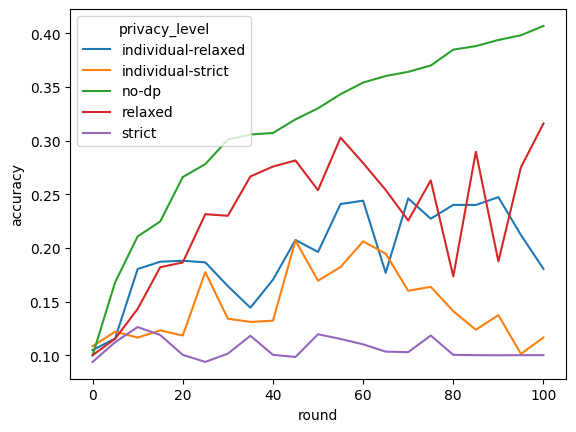
\includegraphics[width=\linewidth]{Bilder/cifar10-accuracy-iid-eps-1-2-3.png}
		\caption{CIFAR-10 (i.i.d.) mit $\epsilon = \{1,2,3\}$}
	\end{subfigure}
	\begin{subfigure}{0.45\textwidth}
		\centering
		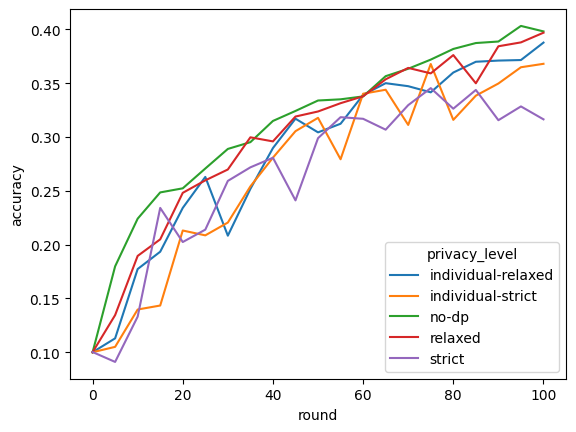
\includegraphics[width=\linewidth]{Bilder/cifar10-accuracy-iid-eps-5-10-20.png}
		\caption{CIFAR-10 (i.i.d.) mit $\epsilon = \{5,10,20\}$}
	\end{subfigure}
	\begin{subfigure}{0.45\textwidth}
		\centering
		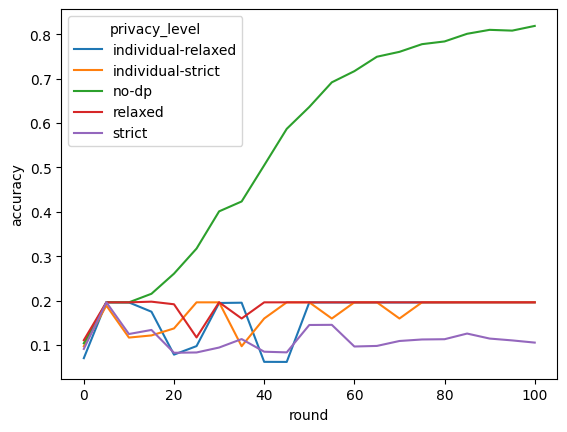
\includegraphics[width=\linewidth]{Bilder/svhn-accuracy-eps-1-2-3.png}
		\caption{SVHN mit $\epsilon = \{1,2,3\}$}
	\end{subfigure}
	\begin{subfigure}{0.45\textwidth}
		\centering
		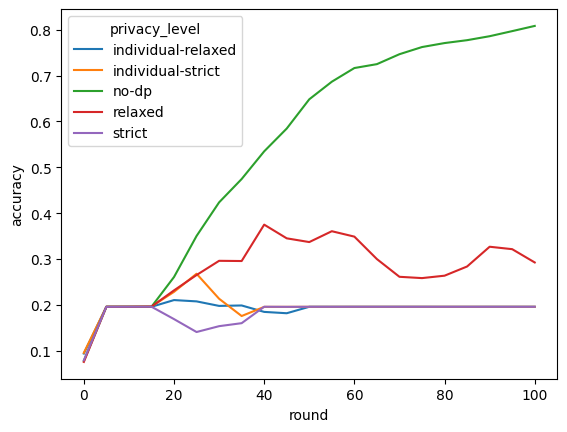
\includegraphics[width=\linewidth]{Bilder/svhn-accuracy-eps-5-10-20.png}
		\caption{SVHN mit $\epsilon = \{5,10,20\}$}
	\end{subfigure}
	\caption{Verlauf der Genauigkeiten auf den Validierungsdaten von CIFAR-10 und SVHN im Training mit kleineren Privacy Budgets}
	\vspace{4in}
	\label{fig:cifar-svhn-small-budgets}
\end{figure}